\begin{comment}
\begin{minipage}{\textwidth}
  \begin{minipage}[b]{0.49\textwidth}
    \begin{figure}[!htb]
\centering
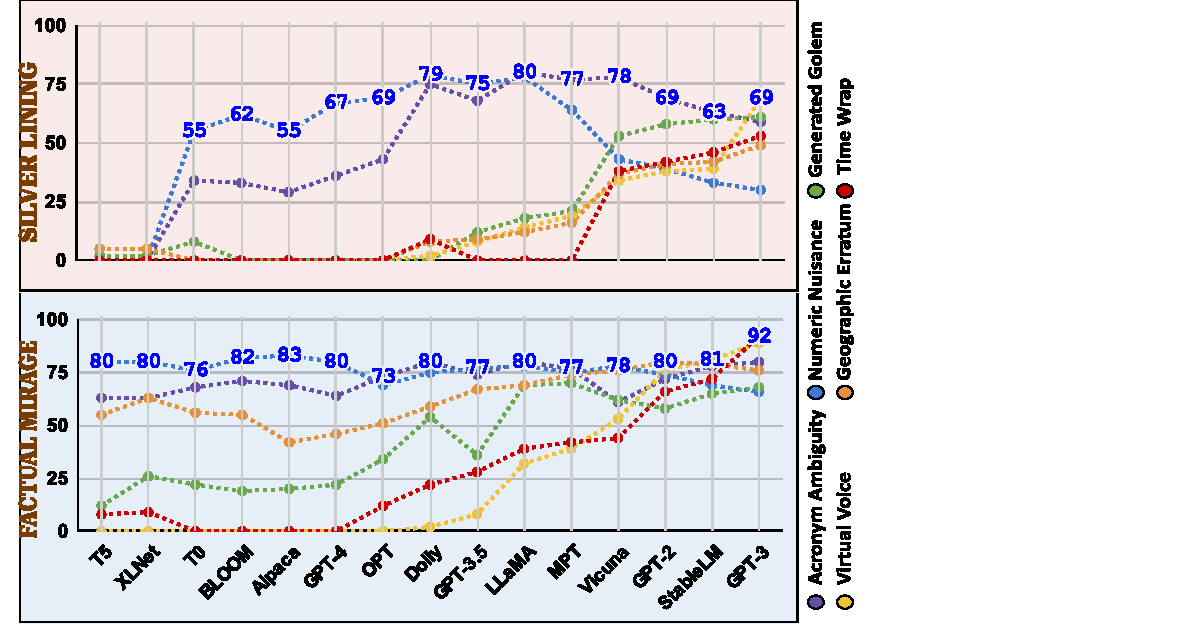
\includegraphics[width=\columnwidth]{img/hvi_all.pdf}
    \caption{Hallucination Vulnerability Index \emph{(HVI)} for different hallucination categories for various LLMs}
\label{fig:hvi}
\end{figure}
  \end{minipage}
  \hfill
  \begin{minipage}[b]{0.49\textwidth}
    %\begin{table}[!ht]
%\tiny
%\centering
%\resizebox{0.32\textheight}{!}{%
\resizebox{0.9\columnwidth}{!}{%
\begin{tabular}{lll}
\toprule
\textbf{LLM} & \textbf{Size} & \textbf{HVI (0-100)}
\\ \midrule
\textbf{GPT-3}    &  175B       &   90 - 
\begin{tikzpicture}
\centering
\draw[red, very thick, fill=red] (0,0)  rectangle (5.62,.1);
\end{tikzpicture}
\\
\textbf{StableLM}    &  7B   &     82 - 
\begin{tikzpicture}
\centering
\draw[red, very thick, fill=red] (0,0)  rectangle (5.12,.1);
\end{tikzpicture}
\\
\textbf{GPT-2}    &   1.5B      &     70 - 
\begin{tikzpicture}
\centering
\draw[red, very thick, fill=red] (0,0)  rectangle (4.38,.1);
\end{tikzpicture}
\\
\textbf{Vicuna}     & 13B      &   62 - 
\begin{tikzpicture}
\centering
\draw[orange, very thick, fill=orange] (0,0)  rectangle (3.88,.1);
\end{tikzpicture}  
\\
\textbf{MPT}    &  7B    &     59 - 
\begin{tikzpicture}
\centering
\draw[orange, very thick, fill=orange] (0,0)  rectangle (3.69,.1);
\end{tikzpicture}   
\\
\textbf{LLaMA}    &  65B    &     57 - 
\begin{tikzpicture}
\centering
\draw[orange, very thick, fill=orange] (0,0)  rectangle (3.56,.1);
\end{tikzpicture}   
\\
\textbf{GPT-3.5}   &    175B      &     53 - 
\begin{tikzpicture}
\centering
\draw[orange, very thick, fill=orange] (0,0)  rectangle (3.31,.1);
\end{tikzpicture}
\\
\textbf{Dolly}    &   12B    &    49 - 
\begin{tikzpicture}
\centering
\draw[violet, very thick, fill=violet] (0,0)  rectangle (3.06,.1);
\end{tikzpicture} 
\\
\textbf{OPT}    &   175B   &     48 - 
\begin{tikzpicture}
\centering
\draw[violet, very thick, fill=violet] (0,0)  rectangle (3,.1);
\end{tikzpicture}   
\\
\textbf{GPT-4}    &   1.7T    &      47 - 
\begin{tikzpicture}
\centering
\draw[violet, very thick, fill=violet] (0,0)  rectangle (2.94,.1);
\end{tikzpicture}  
\\
\textbf{Alpaca}   &   65B    &     40 - 
\begin{tikzpicture}
\centering
\draw[violet, very thick, fill=violet] (0,0)  rectangle (2.5,.1);
\end{tikzpicture}   
\\
\textbf{BLOOM}   &   176B     &   38 - 
\begin{tikzpicture}
\centering
\draw[blue, very thick, fill=blue] (0,0)  rectangle (2.38,.1);
\end{tikzpicture}  
\\
\textbf{T0}    &      11B    &     36 - 
\begin{tikzpicture}
\centering
\draw[blue, very thick, fill=blue] (0,0)  rectangle (2.25,.1);
\end{tikzpicture}  
\\
\textbf{XLNet}   &   340M     &      36 - 
\begin{tikzpicture}
\centering
\draw[blue, very thick, fill=blue] (0,0)  rectangle (2.25,.1);
\end{tikzpicture}  
\\
\textbf{T5}    &    11B      &     32 - 
\begin{tikzpicture}
\centering
\draw[blue, very thick, fill=blue] (0,0)  rectangle (2.0,.1);
\end{tikzpicture}  
\\
% ERNIE           &     40 - \begin{tikzpicture}
% \centering
% \draw[violet, very thick, fill=violet] (0,0)  rectangle (2,.5);
% \end{tikzpicture}  
% \\
% ALBERT          &   33 - \begin{tikzpicture}
% \centering
% \draw[blue, very thick, fill=blue] (0,0)  rectangle (1.8,.5);
% \end{tikzpicture}    
% \\
% DeBERTa         &     32 - \begin{tikzpicture}
% \centering
% \draw[blue, very thick, fill=blue] (0,0)  rectangle (1.6,.5);
% \end{tikzpicture}    
% \\
% ELECTRA         &    32 - \begin{tikzpicture}
% \centering
% \draw[blue, very thick, fill=blue] (0,0)  rectangle (1.8,.5);
% \end{tikzpicture}     
% \\
% RoBERTa         &    28 - \begin{tikzpicture}
% \centering
% \draw[blue, very thick, fill=blue] (0,0)  rectangle (1.4,.5);
% \end{tikzpicture}     
% \\
% BERT            &    26 - \begin{tikzpicture}
% \centering
% \draw[blue, very thick, fill=blue] (0,0)  rectangle (1,.5);
% \end{tikzpicture}     
% \ \ 
\bottomrule
\end{tabular}%
}
%%
%}


%\caption{A ranked list of LLMs based on HVI.}
%\label{tab:LLMs}
%\end{table}
%\vspace{-3mm}









\begin{comment}
%\begin{table}[!ht]
%\tiny
%\centering
\resizebox{\columnwidth}{!}{%
\begin{tabular}{lll}
\toprule
\textbf{LLM} & \textbf{Size} & \textbf{HVI (0-100)}
\\ \midrule
\textbf{GPT 4}    &  N/A       &   90 - 
\begin{tikzpicture}
\centering
\draw[red, very thick, fill=red] (0,0)  rectangle (5,.1);
\end{tikzpicture}
\\
\textbf{GPT 3.5}    &  1.3B   &     82 - 
\begin{tikzpicture}
\centering
\draw[red, very thick, fill=red] (0,0)  rectangle (4.6,.1);
\end{tikzpicture}
\\
\textbf{GPT 3}     & 175B      &   70 - 
\begin{tikzpicture}
\centering
\draw[red, very thick, fill=red] (0,0)  rectangle (4.4,.1);
\end{tikzpicture}  
\\
\textbf{GPT 2}    &   1.5B    &      47 - 
\begin{tikzpicture}
\centering
\draw[red, very thick, fill=red] (0,0)  rectangle (4.2,.1);
\end{tikzpicture}  
\\
\textbf{MPT}   &    7B      &     59 - 
\begin{tikzpicture}
\centering
\draw[orange, very thick, fill=orange] (0,0)  rectangle (4.0,.1);
\end{tikzpicture}
\\
\textbf{OPT}    &   125M      &     59 - 
\begin{tikzpicture}
\centering
\draw[orange, very thick, fill=orange] (0,0)  rectangle (3.8,.1);
\end{tikzpicture}
\\
\textbf{LLaMA}    &   7B    &    52 - 
\begin{tikzpicture}
\centering
\draw[orange, very thick, fill=orange] (0,0)  rectangle (3.5,.1);
\end{tikzpicture} 
\\
\textbf{BLOOM}   &   175B     &   49 - 
\begin{tikzpicture}
\centering
\draw[orange, very thick, fill=orange] (0,0)  rectangle (3.3,.1);
\end{tikzpicture}  
\\
\textbf{Alpaca}    &   7B   &     44 - 
\begin{tikzpicture}
\centering
\draw[orange, very thick, fill=orange] (0,0)  rectangle (3.1,.1);
\end{tikzpicture}   
\\
\textbf{Vicuna}    &  7B    &     44 - 
\begin{tikzpicture}
\centering
\draw[violet, very thick, fill=violet] (0,0)  rectangle (2.9,.1);
\end{tikzpicture}   
\\
\textbf{Dolly}   &   12B    &     44 - 
\begin{tikzpicture}
\centering
\draw[violet, very thick, fill=violet] (0,0)  rectangle (2.7,.1);
\end{tikzpicture}   
\\
\textbf{StableLM}    &  3B    &     44 - 
\begin{tikzpicture}
\centering
\draw[violet, very thick, fill=violet] (0,0)  rectangle (2.5,.1);
\end{tikzpicture}   
\\
\textbf{XLNet}   &   110M     &      42 - 
\begin{tikzpicture}
\centering
\draw[blue, very thick, fill=blue] (0,0)  rectangle (2.3,.1);
\end{tikzpicture}  
\\
\textbf{T0}    &      11B    &     42 - 
\begin{tikzpicture}
\centering
\draw[blue, very thick, fill=blue] (0,0)  rectangle (2.2,.1);
\end{tikzpicture}  
\\
\textbf{T5}    &    3B      &     41 - 
\begin{tikzpicture}
\centering
\draw[blue, very thick, fill=blue] (0,0)  rectangle (2.0,.1);
\end{tikzpicture}  
\\
% ERNIE           &     40 - \begin{tikzpicture}
% \centering
% \draw[violet, very thick, fill=violet] (0,0)  rectangle (2,.5);
% \end{tikzpicture}  
% \\
% ALBERT          &   33 - \begin{tikzpicture}
% \centering
% \draw[blue, very thick, fill=blue] (0,0)  rectangle (1.8,.5);
% \end{tikzpicture}    
% \\
% DeBERTa         &     32 - \begin{tikzpicture}
% \centering
% \draw[blue, very thick, fill=blue] (0,0)  rectangle (1.6,.5);
% \end{tikzpicture}    
% \\
% ELECTRA         &    32 - \begin{tikzpicture}
% \centering
% \draw[blue, very thick, fill=blue] (0,0)  rectangle (1.8,.5);
% \end{tikzpicture}     
% \\
% RoBERTa         &    28 - \begin{tikzpicture}
% \centering
% \draw[blue, very thick, fill=blue] (0,0)  rectangle (1.4,.5);
% \end{tikzpicture}     
% \\
% BERT            &    26 - \begin{tikzpicture}
% \centering
% \draw[blue, very thick, fill=blue] (0,0)  rectangle (1,.5);
% \end{tikzpicture}     
% \\ 
\bottomrule
\end{tabular}%
}
%\caption{A ranked list of LLMs based on HVI.}
%\label{tab:LLMs}
%\end{table}
%\vspace{-3mm}
\end{comment}
    \end{minipage}
  \end{minipage}
\end{comment}

\vspace{-1mm}
\section{\textls[-10]{Hallucination Vulnerability Index (HVI)}}
\label{sec:hvi}
\vspace{-2mm}
Given the growing usage of LLMs and their likeliness to hallucinate, there exists no uniform evaluation metric to measure these LLMs' hallucinations. To address this gap, we define \textbf{HVI}, a comparative spectrum that allows us to evaluate and rank LLMs based on their vulnerability to producing hallucinations. HVI is calculated as in \cref{eq:eq1}:

\vspace{-8mm}
%% \renewcommand{\theequation}{\arabic{equation}}
% \renewcommand{\theequation*}{\arabic{equation*}}
%v\begin{equation*}
%v\begin{aligned}
%\resizebox{\hsize}{!}{$%
% \resizebox{0.89\hsize}{!}{
%vHVI_x=\frac{100}{U*2}\left[\sum_{x=1}^U(N(x)-P(E F M)) \times \left(1-\frac{P(E F M)}{N(x)}+ \\
%v\delta_1(x)\right)+(N(x)-P(E S L))\times \left(1-\frac{P(E S L)}{N(x)}+\delta_2(x)\right)\right]
% }
% }
% \tag{\theequation*}
%v\label{eq:eq1}
%v\end{aligned}
%v\end{equation*}

%   \begin{equation*}
%   \begin{aligned}
% HVI_x=\frac{100}{U*2}\left[ \sum_{x=1}^U(N(x)-P(E F M)) \times \left(1-\frac{P(E F M)}{N(x)}+ \\
% \delta_1(x)\right)+(N(x)-P(E S L))\times \left(1-\frac{P(E S L)}{N(x)}+\delta_2(x)\right)\right]
%    \end{aligned}
% \end{equation*}


\begin{equation} \nonumber
    \label{eq:eq1}
 \Scale[0.8]{HVI_x = \frac{100}{U*2}\left[ \sum_{x=1}^U(N(x)-P(E F M)) *\left(1-\frac{P(E F M)}{N(x)}+\delta_1(x)\right)+ \right.} \\
\Scale[0.8]{\left. (N(x)-P(E S L))\left(1-\frac{P(E S L)}{N(x)}+\delta_2(x)\right)\right]}
\end{equation}

\begin{equation} \nonumber
 \Scale[0.8]{HVI_x = \frac{100}{U*2}\left[ \sum_{x=1}^U(N(x)-N(E F M)) *\left(1-P(E F M)+\delta_1\right)+ \right.} \\
\Scale[0.8]{\left. (N(x)-N(E S L))*\left(1-P(E S L)+\delta_2\right)\right]}
\label{eq:eq1}
\end{equation}

\vspace{-3mm}

\noindent
When defining HVI, we take several factors into account. Firstly, not all sentences generated by an LLM are hallucinated, so it is important to determine the ratio of actual hallucinated sentences with the total number of sentences. In this context, we consider $U$ as the total number of sentences and $N(x)$ as the total number of hallucinated sentences produced by an LLM. Secondly, LLMs can exhibit different characteristics, such as higher EFM or ESL tendencies, or they can have varying levels of overall hallucination. This notion is captured by introducing the terms {$N(x)-N(EFM)$} and {$N(x)-N(ESL)$} in the equation. It is worth noting that we did not consider variations of intrinsic hallucinations in HVI calculation, as they are relatively minor and exhibit lower vulnerability overall. Lastly, comparative measures are needed to rank LLMs based on their vulnerability to hallucination. This is achieved using multiplicative damping factors, $\delta_1$ and $\delta_2$, which are calculated based on $\mu \pm rank_x \times \sigma$. Initially, we calculate the HVI for all 15 LLMs, considering $\delta_1$ and $\delta_2$ as zero. With these initial HVIs, we obtain the mean ($\mu$) and standard deviation ($\sigma$), allowing us to recalculate the HVIs for all the LLMs. The resulting HVIs are then ranked and scaled providing a comparative spectrum as presented in \cref{tab:hvi_spectrum}, similar to z-score normalization \cite{Normalization-z} and/or min-max normalization \cite{Normalization-min}. Having damping factors enables easy exponential smoothing with a handful of data points, 15 in this case. Finally, for ease of interpretability, HVI is scaled between $0-100$.

\vspace{-3mm}
\begin{figure}[h]
\centering
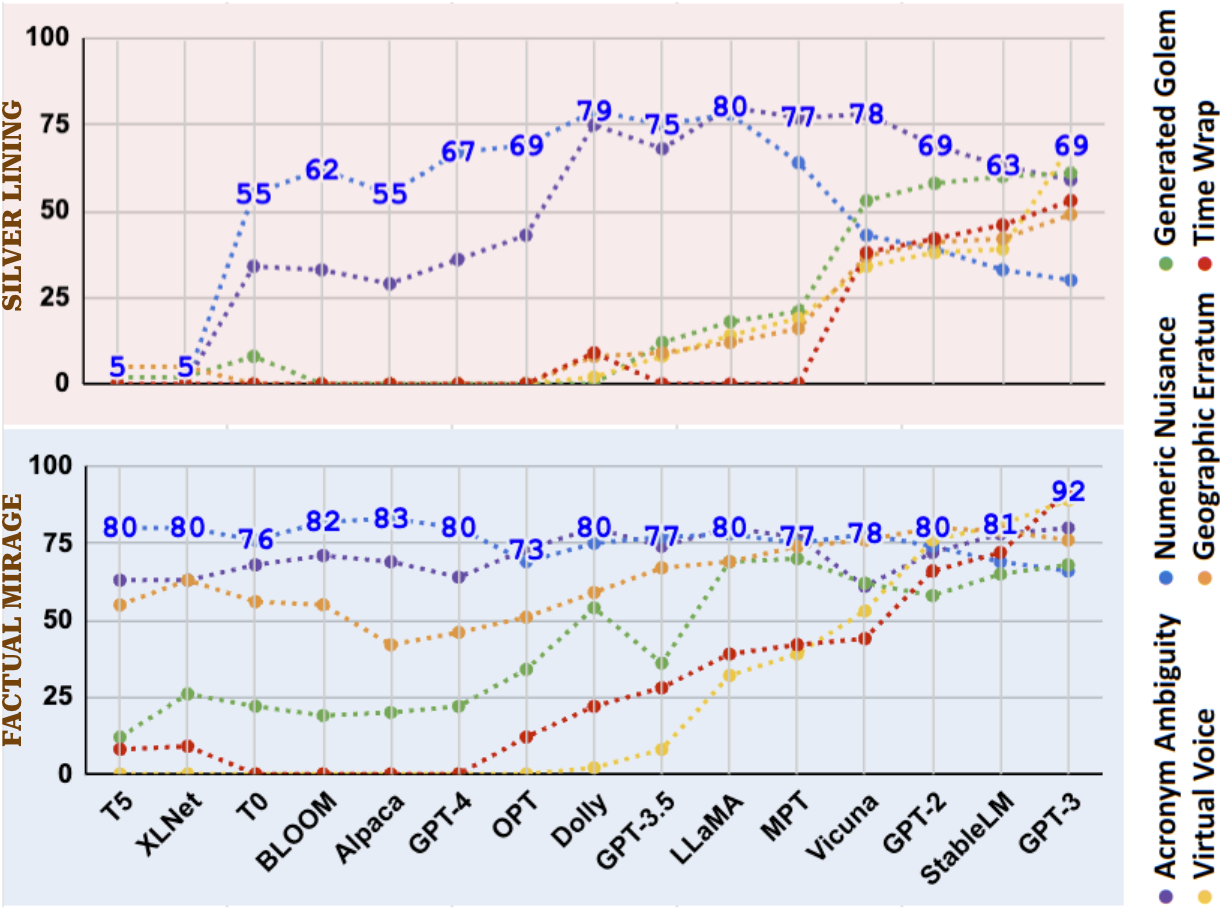
\includegraphics[width=0.9\columnwidth]{img/hvi_all.png}
\vspace{-2mm}
  \caption{HVI for different hallucination categories across various LLMs.}
  \label{fig:hvi-cat}
  %\vspace{-2mm}
\end{figure}

\vspace{-5mm}
\begin{figure}[h]
\minipage{0.4\textwidth}
\centering
%\begin{table}[!ht]
%\tiny
%\centering
%\resizebox{0.32\textheight}{!}{%
\resizebox{0.9\columnwidth}{!}{%
\begin{tabular}{lll}
\toprule
\textbf{LLM} & \textbf{Size} & \textbf{HVI (0-100)}
\\ \midrule
\textbf{GPT-3}    &  175B       &   90 - 
\begin{tikzpicture}
\centering
\draw[red, very thick, fill=red] (0,0)  rectangle (5.62,.1);
\end{tikzpicture}
\\
\textbf{StableLM}    &  7B   &     82 - 
\begin{tikzpicture}
\centering
\draw[red, very thick, fill=red] (0,0)  rectangle (5.12,.1);
\end{tikzpicture}
\\
\textbf{GPT-2}    &   1.5B      &     70 - 
\begin{tikzpicture}
\centering
\draw[red, very thick, fill=red] (0,0)  rectangle (4.38,.1);
\end{tikzpicture}
\\
\textbf{Vicuna}     & 13B      &   62 - 
\begin{tikzpicture}
\centering
\draw[orange, very thick, fill=orange] (0,0)  rectangle (3.88,.1);
\end{tikzpicture}  
\\
\textbf{MPT}    &  7B    &     59 - 
\begin{tikzpicture}
\centering
\draw[orange, very thick, fill=orange] (0,0)  rectangle (3.69,.1);
\end{tikzpicture}   
\\
\textbf{LLaMA}    &  65B    &     57 - 
\begin{tikzpicture}
\centering
\draw[orange, very thick, fill=orange] (0,0)  rectangle (3.56,.1);
\end{tikzpicture}   
\\
\textbf{GPT-3.5}   &    175B      &     53 - 
\begin{tikzpicture}
\centering
\draw[orange, very thick, fill=orange] (0,0)  rectangle (3.31,.1);
\end{tikzpicture}
\\
\textbf{Dolly}    &   12B    &    49 - 
\begin{tikzpicture}
\centering
\draw[violet, very thick, fill=violet] (0,0)  rectangle (3.06,.1);
\end{tikzpicture} 
\\
\textbf{OPT}    &   175B   &     48 - \begin{tikzpicture}
\centering
\draw[violet, very thick, fill=violet] (0,0)  rectangle (3,.1);
\end{tikzpicture}   
\\
\textbf{GPT-4}    &   1.7T    &      47 - \begin{tikzpicture}
\centering
\draw[violet, very thick, fill=violet] (0,0)  rectangle (2.94,.1);
\end{tikzpicture}  
\\
\textbf{Alpaca}   &   65B    &     40 - \begin{tikzpicture}
\centering
\draw[violet, very thick, fill=violet] (0,0)  rectangle (2.5,.1);
\end{tikzpicture}   
\\
\textbf{BLOOM}   &   176B     &   38 - \begin{tikzpicture}
\centering
\draw[blue, very thick, fill=blue] (0,0)  rectangle (2.38,.1);
\end{tikzpicture}  
\\
\textbf{T0}    &      11B    &     36 - \begin{tikzpicture}
\centering
\draw[blue, very thick, fill=blue] (0,0)  rectangle (2.25,.1);
\end{tikzpicture}  
\\
\textbf{XLNet}   &   340M     &      36 - \begin{tikzpicture}
\centering
\draw[blue, very thick, fill=blue] (0,0)  rectangle (2.25,.1);
\end{tikzpicture}  
\\
\textbf{T5}    &    11B      &     32 - \begin{tikzpicture}
\centering
\draw[blue, very thick, fill=blue] (0,0)  rectangle (2.0,.1);
\end{tikzpicture}  
\\
% ERNIE           &     40 - \begin{tikzpicture}
% \centering
% \draw[violet, very thick, fill=violet] (0,0)  rectangle (2,.5);
% \end{tikzpicture}  
% \\
% ALBERT          &   33 - \begin{tikzpicture}
% \centering
% \draw[blue, very thick, fill=blue] (0,0)  rectangle (1.8,.5);
% \end{tikzpicture}    
% \\
% DeBERTa         &     32 - \begin{tikzpicture}
% \centering
% \draw[blue, very thick, fill=blue] (0,0)  rectangle (1.6,.5);
% \end{tikzpicture}    
% \\
% ELECTRA         &    32 - \begin{tikzpicture}
% \centering
% \draw[blue, very thick, fill=blue] (0,0)  rectangle (1.8,.5);
% \end{tikzpicture}     
% \\
% RoBERTa         &    28 - \begin{tikzpicture}
% \centering
% \draw[blue, very thick, fill=blue] (0,0)  rectangle (1.4,.5);
% \end{tikzpicture}     
% \\
% BERT            &    26 - \begin{tikzpicture}
% \centering
% \draw[blue, very thick, fill=blue] (0,0)  rectangle (1,.5);
% \end{tikzpicture}     
% \ \ 
\bottomrule
\end{tabular}%
}
%%
%}


%\caption{A ranked list of LLMs based on HVI.}
%\label{tab:LLMs}
%\end{table}
%\vspace{-3mm}









\begin{comment}
%\begin{table}[!ht]
%\tiny
%\centering
\resizebox{\columnwidth}{!}{%
\begin{tabular}{lll}
\toprule
\textbf{LLM} & \textbf{Size} & \textbf{HVI (0-100)}
\\ \midrule
\textbf{GPT 4}    &  N/A       &   90 - \begin{tikzpicture}
\centering
\draw[red, very thick, fill=red] (0,0)  rectangle (5,.1);
\end{tikzpicture}
\\
\textbf{GPT 3.5}    &  1.3B   &     82 - \begin{tikzpicture}
\centering
\draw[red, very thick, fill=red] (0,0)  rectangle (4.6,.1);
\end{tikzpicture}
\\
\textbf{GPT 3}     & 175B      &   70 - \begin{tikzpicture}
\centering
\draw[red, very thick, fill=red] (0,0)  rectangle (4.4,.1);
\end{tikzpicture}  
\\
\textbf{GPT 2}    &   1.5B    &      47 - \begin{tikzpicture}
\centering
\draw[red, very thick, fill=red] (0,0)  rectangle (4.2,.1);
\end{tikzpicture}  
\\
\textbf{MPT}   &    7B      &     59 - \begin{tikzpicture}
\centering
\draw[orange, very thick, fill=orange] (0,0)  rectangle (4.0,.1);
\end{tikzpicture}
\\
\textbf{OPT}    &   125M      &     59 - \begin{tikzpicture}
\centering
\draw[orange, very thick, fill=orange] (0,0)  rectangle (3.8,.1);
\end{tikzpicture}
\\
\textbf{LLaMA}    &   7B    &    52 - \begin{tikzpicture}
\centering
\draw[orange, very thick, fill=orange] (0,0)  rectangle (3.5,.1);
\end{tikzpicture} 
\\
\textbf{BLOOM}   &   175B     &   49 - \begin{tikzpicture}
\centering
\draw[orange, very thick, fill=orange] (0,0)  rectangle (3.3,.1);
\end{tikzpicture}  
\\
\textbf{Alpaca}    &   7B   &     44 - \begin{tikzpicture}
\centering
\draw[orange, very thick, fill=orange] (0,0)  rectangle (3.1,.1);
\end{tikzpicture}   
\\
\textbf{Vicuna}    &  7B    &     44 - \begin{tikzpicture}
\centering
\draw[violet, very thick, fill=violet] (0,0)  rectangle (2.9,.1);
\end{tikzpicture}   
\\
\textbf{Dolly}   &   12B    &     44 - \begin{tikzpicture}
\centering
\draw[violet, very thick, fill=violet] (0,0)  rectangle (2.7,.1);
\end{tikzpicture}   
\\
\textbf{StableLM}    &  3B    &     44 - \begin{tikzpicture}
\centering
\draw[violet, very thick, fill=violet] (0,0)  rectangle (2.5,.1);
\end{tikzpicture}   
\\
\textbf{XLNet}   &   110M     &      42 - \begin{tikzpicture}
\centering
\draw[blue, very thick, fill=blue] (0,0)  rectangle (2.3,.1);
\end{tikzpicture}  
\\
\textbf{T0}    &      11B    &     42 - \begin{tikzpicture}
\centering
\draw[blue, very thick, fill=blue] (0,0)  rectangle (2.2,.1);
\end{tikzpicture}  
\\
\textbf{T5}    &    3B      &     41 - \begin{tikzpicture}
\centering
\draw[blue, very thick, fill=blue] (0,0)  rectangle (2.0,.1);
\end{tikzpicture}  
\\
% ERNIE           &     40 - \begin{tikzpicture}
% \centering
% \draw[violet, very thick, fill=violet] (0,0)  rectangle (2,.5);
% \end{tikzpicture}  
% \\
% ALBERT          &   33 - \begin{tikzpicture}
% \centering
% \draw[blue, very thick, fill=blue] (0,0)  rectangle (1.8,.5);
% \end{tikzpicture}    
% \\
% DeBERTa         &     32 - \begin{tikzpicture}
% \centering
% \draw[blue, very thick, fill=blue] (0,0)  rectangle (1.6,.5);
% \end{tikzpicture}    
% \\
% ELECTRA         &    32 - \begin{tikzpicture}
% \centering
% \draw[blue, very thick, fill=blue] (0,0)  rectangle (1.8,.5);
% \end{tikzpicture}     
% \\
% RoBERTa         &    28 - \begin{tikzpicture}
% \centering
% \draw[blue, very thick, fill=blue] (0,0)  rectangle (1.4,.5);
% \end{tikzpicture}     
% \\
% BERT            &    26 - \begin{tikzpicture}
% \centering
% \draw[blue, very thick, fill=blue] (0,0)  rectangle (1,.5);
% \end{tikzpicture}     
% \\ 
\bottomrule
\end{tabular}%
}
%\caption{A ranked list of LLMs based on HVI.}
%\label{tab:LLMs}
%\end{table}
%\vspace{-3mm}
\end{comment}
\vspace{-2mm}
\caption{The HVI scale illustrates the hallucination tendencies exhibited by various LLMs.}
  \label{tab:hvi_spectrum}
\endminipage
\minipage{0.05\textwidth}
\vspace{-17mm}
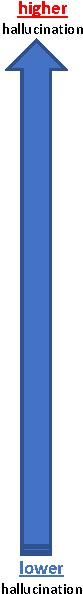
\includegraphics[height=4.5cm]{img/hvi_arrow.pdf}
\endminipage
\vspace{-4.5mm}
\end{figure}


% \vspace{-2mm}
\begin{figure*}[!ht]
\centering
\minipage{\textwidth}
% \minipage{\textwidth}
% \begin{table*}[!ht]%[H]
\vspace{-1mm}
\resizebox{0.98\textwidth}{!}{%
\begin{tabular}{p{0.06\textwidth}|p{1.5\textwidth}} \toprule
{\footnotesize \textbf{Prompt}} 
& \footnotesize\textit{USA's stance on Ukraine Russia war} \\ \hline
\rotatebox[origin=r]{90}{\parbox[c]{2cm}{\centering {\footnotesize \textbf{Hallucinated text}}}}
& 
{\footnotesize The official stance of the \colorbox{LightBlue}{United States} on the \colorbox{LightBlue}{Russia-Ukraine} war has been consistent in supporting \colorbox{LightBlue}{Ukraine's sovereignty, territorial integrity, and the peaceful resolution} of the conflict. The \colorbox{LightBlue}{U.S.} has \colorbox{LightBlue}{condemned Russia's actions} in \colorbox{LightBlue}{annexing Crimea} and its support for separatist movements in eastern \colorbox{LightBlue}{Ukraine}. Despite maintaining a \colorbox{LightBlue}{diplomatic} stance, \colorbox{pink}{the U.S. President Barack Obama} stated that the \colorbox{LightBlue}{United States} would not deploy troops to \colorbox{LightBlue}{Ukraine}. Additionally, this lack of support extends to the withholding of financial and \colorbox{LightBlue}{military assistance}, including \colorbox{LightBlue}{military equipment}, \colorbox{LightBlue}{training}, and \colorbox{LightBlue}{advisory support}. This \colorbox{pink}{sentiment was reiterated} by \colorbox{pink}{Paul Altman} during a press review at the \colorbox{LightBlue}{White House}...} \\ \hline
\rotatebox[origin=r]{90}{\parbox[c]{2cm}{\centering {\footnotesize \textbf{Mitigated text\\\textcolor{blue}{ENTROPY\textsubscript{BB}}}}}}
& 
\footnotesize The official stance of the \colorbox{Thistle}{government} on the \colorbox{Thistle}{ongoing} war has been consistent in supporting \colorbox{Thistle}{resolution} of the conflict. The \colorbox{Thistle}{government} has \colorbox{Thistle}{condemned Russia} in \colorbox{Thistle}{country} and its support for separatist movements in eastern \colorbox{Thistle}{country}. Despite maintaining a \colorbox{Thistle}{neutral} stance, the \colorbox{Thistle}{government} stated that the \colorbox{Thistle}{country} would not deploy troops to \colorbox{Thistle}{unknown}. Additionally, this lack of support extends to the withholding of financial and \colorbox{Thistle}{resources}, including \colorbox{Thistle}{administrative}, \colorbox{Thistle}{technical}, and \colorbox{Thistle}{legal}. This sentiment was \colorbox{Thistle}{echoed} by \colorbox{Thistle}{minister} during a press review at the \colorbox{Thistle}{conference}... \\ \hline
\rotatebox[origin=r]{90}{\parbox[c]{2.5cm}{\centering {\footnotesize \textbf{Edit Suggestions\\\textcolor{blue}{FACTUALITY\textsubscript{GB}}}}}}
& 
\footnotesize The official stance of the United States on the Russia-Ukraine war has been consistent in supporting Ukraine's sovereignty, territorial integrity, and the peaceful resolution of the conflict. The U.S. has condemned Russia's actions in annexing Crimea and its support for separatist movements in eastern Ukraine. \colorbox{PeachPuff}{Despite maintaining a diplomatic stance, U.S. President Barack Obama stated that the United States would not deploy troops to Ukraine.}\colorbox{Khaki}{Additionally, this lack of support extends to the} \colorbox{Khaki}{withholding of financial and military assistance, including military equipment, training, and advisory support.} \colorbox{PeachPuff}{This sentiment was reiterated by Paul Altman during a press review at the} \colorbox{PeachPuff}{White House}... \\ \bottomrule
\end{tabular}%
}
\vspace{-2mm}
\caption{A hallucination example pre- and post-mitigation. \colorbox{pink}{A} - hallucinated fragments, \colorbox{LightBlue}{B} - high entropy fragments, \colorbox{Thistle}{C} - replaced text, \colorbox{Khaki}{D} - highlighted text for no information found, and \colorbox{PeachPuff}{E} - refuted text fragments by textual entailment. ~\cref{sec:mitigation_appendix} contains more examples.} 
\label{tab:hallucination_ex}
\endminipage
\newline
\centering
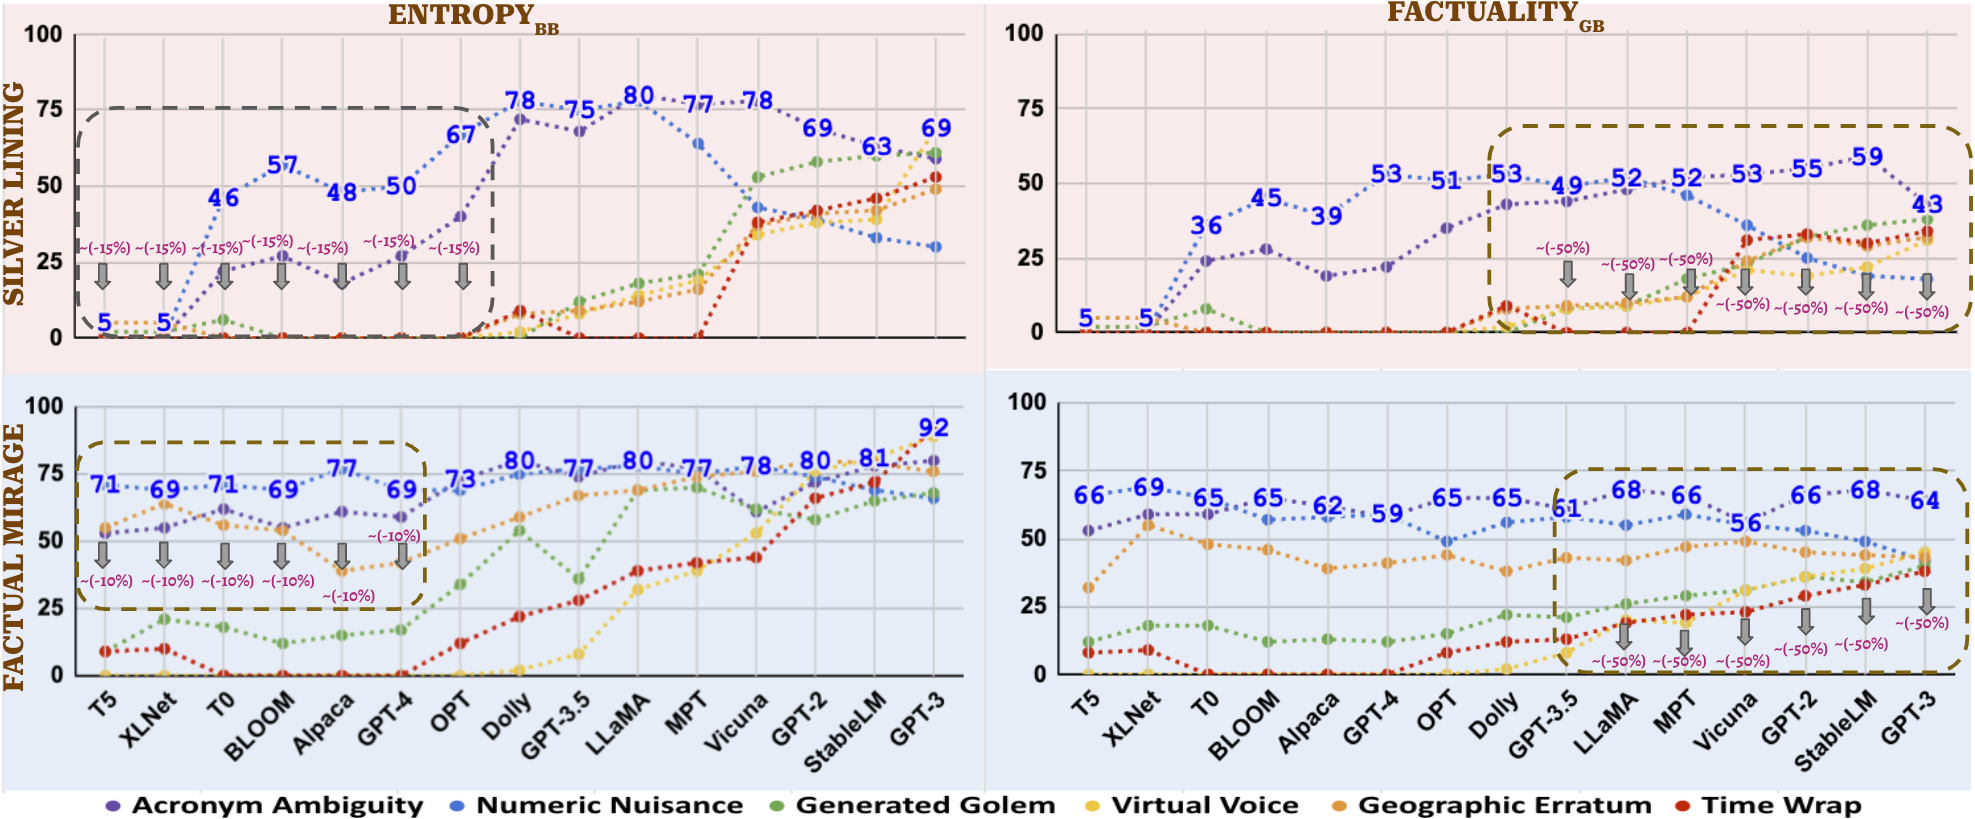
\includegraphics[width=\textwidth, height=7.2cm]{img/mitigation_all.png}
\vspace{-5mm}
\caption{\textls[-10]{Impact of mitigation techniques across the various categories and types of hallucination. For details on the evaluation strategy, i.e., the process of identifying the degree of hallucination after mitigation, cf. \cref{sec:eval_strategy}.}}
    \label{fig:mitigation_all}
%\vspace{-5mm}
\end{figure*}

%\vspace{-1mm}
%\begin{tcolorbox}
%[ left=9pt,right=2pt,
%colback=teal!5!white,colframe=teal!75!black,colbacktitle=teal,
%  title=\footnotesize \selectfont \textbf{\textsc{Implications derived from HVI}} ]

\begin{tcolorbox}[
left=9pt,right=2pt,colback=teal!5!white,colframe=teal!75!black,colbacktitle=teal,
  title=\footnotesize \fontfamily{qbk} \selectfont \textbf{Implications derived from HVI} ]
  
\vspace{-2mm}
\begin{itemize}
\setlength\itemsep{0em}
\begin{spacing}{0.85}

\begin{comment}
\item[\ding{224}] 
{\footnotesize 
{\fontfamily{phv}\fontsize{8}{9}
%\begin{spacing}{1}
\selectfont
A positive correlation exists between the increased LLM size and a higher likelihood of hallucination, as indicated in Table \ref{tab:LLMs}. Further supporting evidence can be found in Appendix \ref{sec:appendix}.
}
%\end{spacing}
}
\end{comment}

\item[\ding{224}] 
{\footnotesize 
{\fontfamily{phv}\fontsize{8}{9}
%\begin{spacing}{1}
\selectfont
Larger LLMs without RLHF \cite{DBLP:journals/corr/abs-1909-08593} are prone to both orientations of hallucination, as shown in ~\cref{tab:hvi_spectrum}. To inspect the categorical changes in hallucination behavior for a particular LLM, please refer to the vertical axis of the HVI spectrum.
}
%\end{spacing}
}

\item[\ding{224}] 
{\footnotesize 
{\fontfamily{phv}\fontsize{8}{9}
%\begin{spacing}{1}
\selectfont
%Per our definitions, Numeric Nuisance and Acronym Ambiguity are relatively mild categories of hallucination. These categories exhibit a decrease in SL orientation as the LLM size increases. Conversely, more complex hallucination categories such as Time Wrap and Geographic Erratum tend to increase in prevalence. It is worth noting that Virtual Voice shows a significant jump from GPT-3.5 to GPT-4.
As per our definitions, Numeric Nuisance and Acronym Ambiguity are mild hallucination categories, showing reduced SL orientation as LLM size grows. Conversely, complex categories like Time Wrap and Geographic Erratum become more prevalent. Notably, Virtual Voice significantly increases from GPT-3.5 to GPT-4.
}
%\end{spacing}
}

\item[\ding{224}] 
{\footnotesize 
{\fontfamily{phv}\fontsize{8}{9}
%\begin{spacing}{1}
\selectfont
%For LLMs below a certain size threshold, namely T5, Dolly, etc., hallucination categories such as Generated Golem, Virtual Voice, and Geographic Erratum exhibit negligible occurrences.
For smaller LLMs like T5, Dolly, etc., Generated Golem, Virtual Voice, and Geographic Erratum categories of hallucination are rarely observed.
}
%\end{spacing}
}
%\end{spacing}

\vspace{-6mm}
\end{spacing}
\end{itemize}
\end{tcolorbox}
\vspace{-2mm}


%\begin{figure}[!htb]
\centering
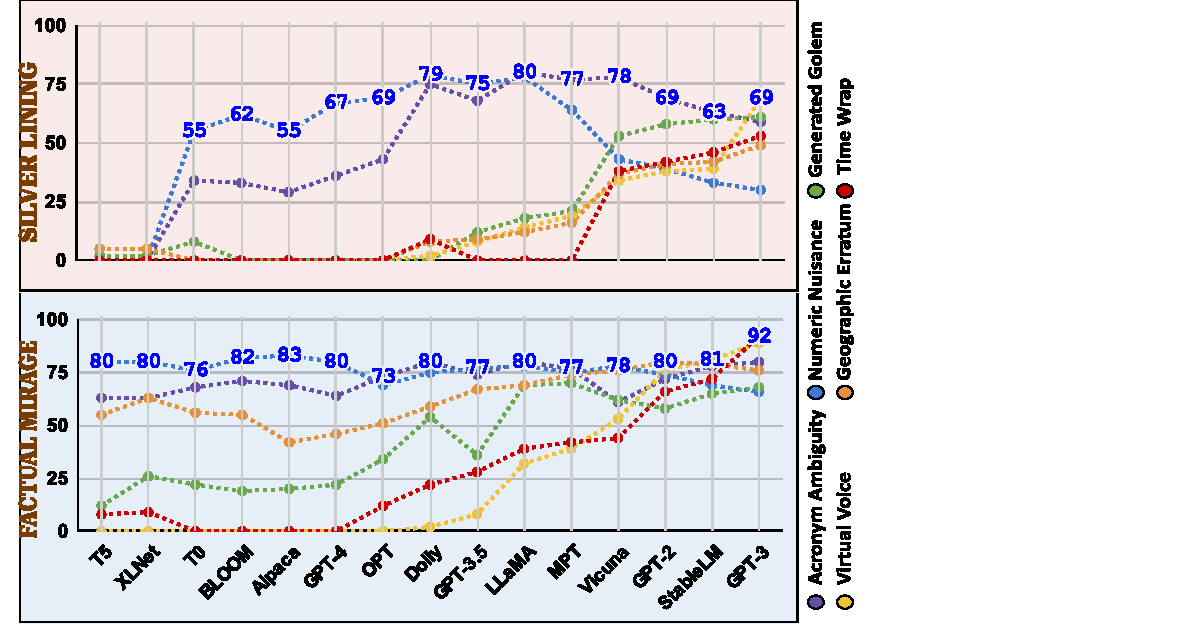
\includegraphics[width=\columnwidth]{img/hvi_all.pdf}
    \caption{Hallucination Vulnerability Index \emph{(HVI)} for different hallucination categories for various LLMs}
\label{fig:hvi}
\end{figure}







%\adt{When defining HVI thre are quite a few factors to keep in mind - i) not all the sentences produced by an LLM are hallucinated, therefore we need a ratio to understand how many sentences are actually hallucinated; $U$ is total number of sentences, $N(x)$ is the total number of hallucinated sentences by an LLM, ii) An LLM can pose different charracteristics, can possess higher EFM than ESL or reverse or else can possess lower hallucination overall. To capture such notions $N(x)-P(EFM)$ and $N(x)-P(ESL)$ are added in the equation. iii) lastly, we need comparative measures to rank various LLM based on their hallucination vulnerability. $\delta_1(x)$ and $\delta_2(x)$ are multiplicative damping factors given by $\mu \pm rank \times \sigma$. First we calculate HVI for all the 15 LLMs considering $\delta_1(x)$ and $\delta_2(x)$ as zero. Having all the HVIs from all the LLMs we obtain $\mu$ and $\sigma$ and recalcualate HVIs for all the LLMs. Resultant HVIs are ranked and potrays a comparative measure as reported in the \cref{tab:LLMs}.}

%as a score to quantify the hallucination for different LLMs listed in \cref{tab:LLMs}. In \cref{eq:eq1}, we define HVI as ...


%\vspace{-2mm}
%


\begin{figure*}[ht!]
\centering
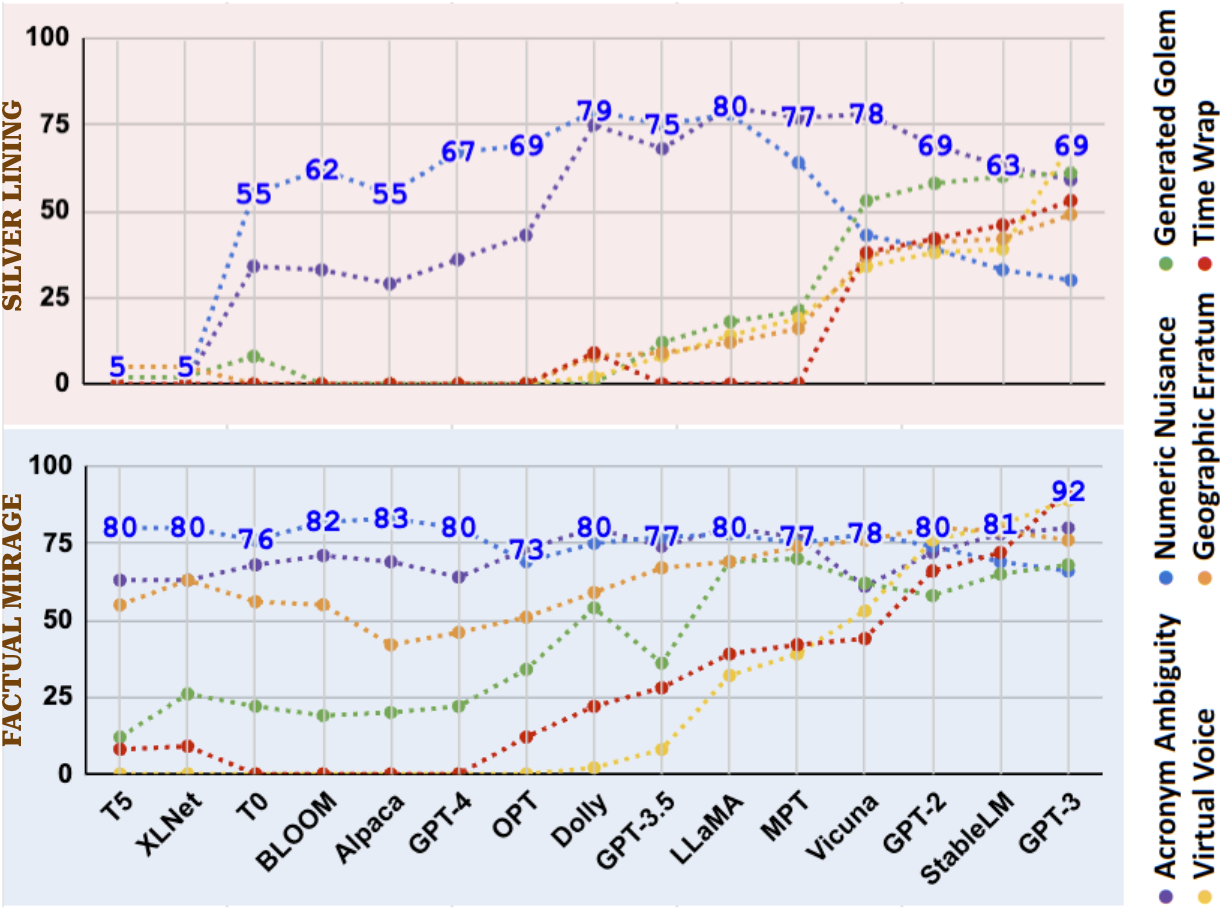
\includegraphics[width=\textwidth]{img/hvi_all.png}
\label{fig:hvi_all}
\end{figure*}



\begin{comment}
\begin{figure*}[!htb]
\minipage{0.5\textwidth}
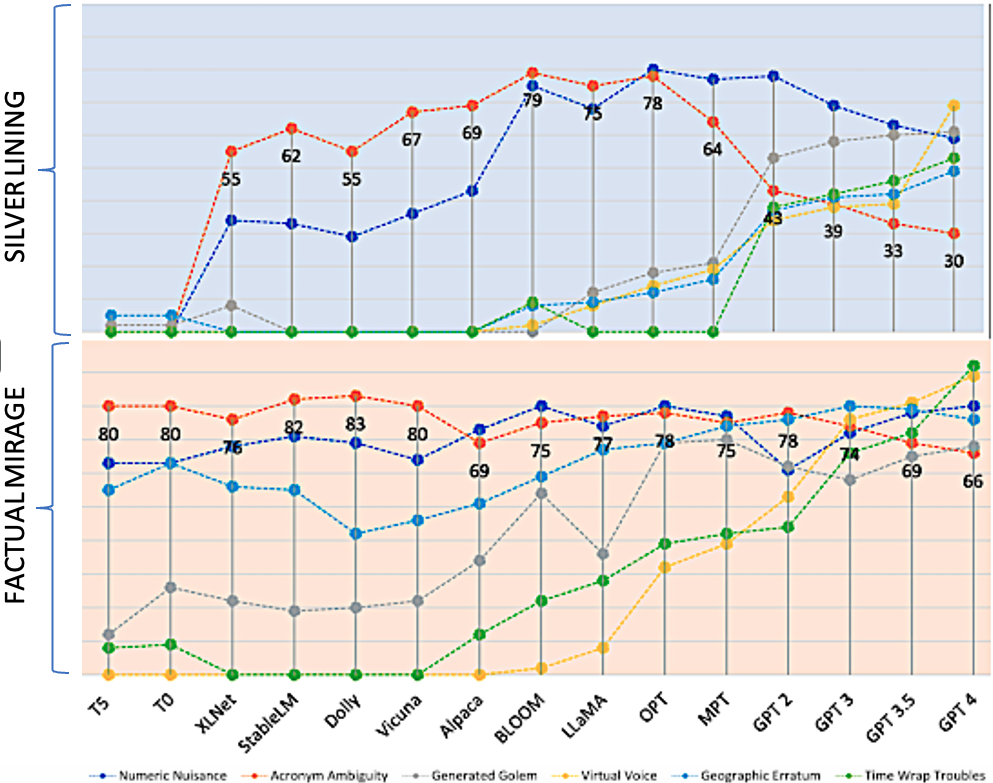
\includegraphics[width=\columnwidth]{img/hvi-final.png}
  \caption{Results after mitigation technique 1}
  \label{fig:awesome_image1}
\endminipage\hfill
\minipage{0.46\textwidth}
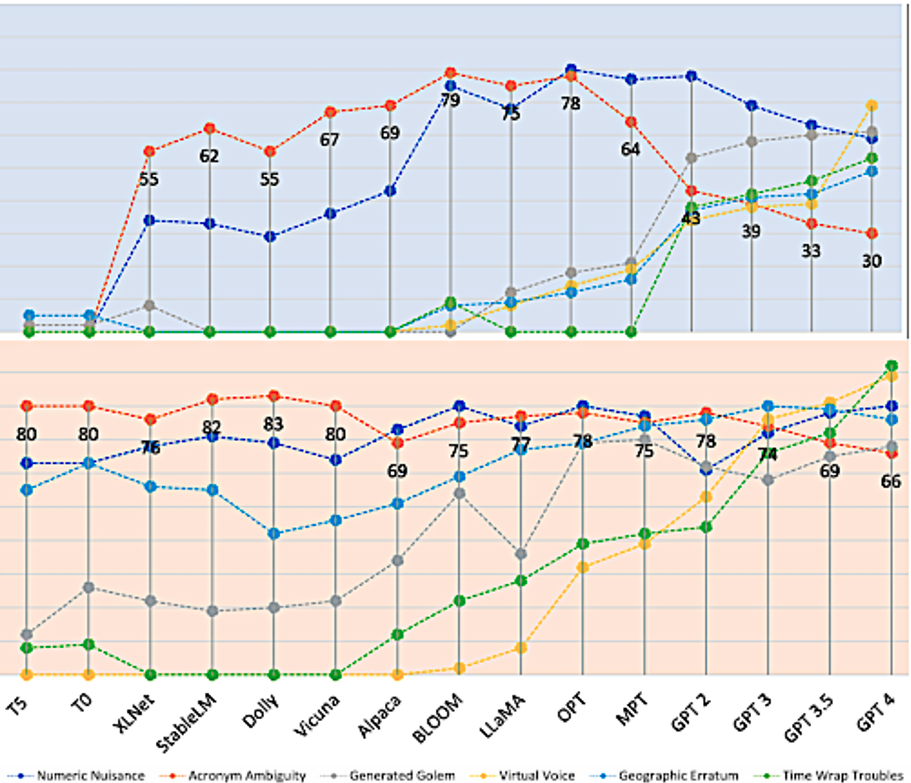
\includegraphics[width=\columnwidth]{img/hvi-final_1.png}
  \caption{Results after mitigation technique 2}
  \label{fig:awesome_image2}
\endminipage
\end{figure*}
\end{comment}










\begin{comment}
\subsection{Why and where LLMs hallucinate?}
where LLMs hallucinate? as in?? you mean the high entropy points?

\subsection{High entropy points}
``High entropy points'' in a language model as the points where the probability distribution of the language model assigns high probabilities to many possible next tokens or words, indicating uncertainty or ambiguity in the model's predictions. In other words, high entropy points are those where the model is unable to determine with high confidence what the next word in a sentence should be based on the context. This can occur due to various factors, such as lack of relevant training data or the presence of multiple plausible interpretations for a given context.

\subsection{Burstiness}
``Burstiness'' in a language model can be defined as a phenomenon where certain words or phrases occur much more frequently in a given text or corpus than others, leading to uneven or ``bursty'' distribution of word occurrences. This phenomenon is often observed in natural language text, where certain words or phrases tend to appear in specific contexts or topics, leading to their over-representation in those contexts or topics. Burstiness can be a challenge for language models, as they need to be able to capture the varying frequencies of word occurrences in different contexts and account for the impact of bursty words on the overall language distribution.

\subsection{Readability}
``Readability'' in a language model is the ability to generate text that is easy to understand and comprehend by human readers. A language model that produces text that is easy to read and understand can be considered to have high readability. Factors that can affect the readability of a language model include its vocabulary and grammar, the complexity of its output, the coherence of its text, and the relevance of its content to the given task or context. Readability is an important aspect of natural language processing, as it determines the degree to which the generated text can be effectively used and understood by humans.
\end{comment}